% Fallunterscheidung bei RLC-Serienschwingkreis, Nullstellen
% Eigenwerte (Nullstellen) im komplexen Zahlenraum (Ortskurve nach D)
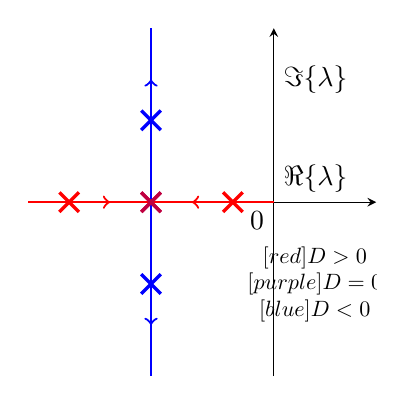
\begin{tikzpicture}[x=1cm,y=1cm]
\begin{axis}[
    axis lines=middle,
    xmin=-3, xmax=1.25,
    ymin=-2.125, ymax=2.125,
    %xlabel={$\Re\{\lambda\}$},
    %ylabel={$\Im\{\lambda\}$},
    ticks=none,
    grid=none,
    width=6cm,
    height=6cm,
]
    % Achsen-Beschriftung
    \node[below left] at (0,0) {0};
    \node[above right] at (0,0) {$\Re\{\lambda\}$};
    \node[right] at (0,1.5) {$\Im\{\lambda\}$};

    % Ortskurven Verlauf
    \draw[thick, draw=red, -] (-3.0,0) -- (-1.5,0);         \draw[thick, draw=red, ->] (-3.0,0) -- (-2.0,0);    % OK aperiodisch
    \draw[thick, draw=red, -] (-0.0,0) -- (-1.5,0);         \draw[thick, draw=red, ->] (-0.0,0) -- (-1.0,0);    % OK aperiodisch
    \draw[thick, draw=blue,-] (-1.5,0) -- (-1.5,-2.125);    \draw[thick, draw=blue,->] (-1.5,0) -- (-1.5,-1.5); % OK periodisch
    \draw[thick, draw=blue,-] (-1.5,0) -- (-1.5,+2.125);    \draw[thick, draw=blue,->] (-1.5,0) -- (-1.5,+1.5); % OK periodisch

    % Nullstellen
    \addplot[very thick, mark size=5pt, mark=x, color=red, draw=none]    coordinates {(-2.5,0) (-0.5,0)}; % NST aperiodisch
    \addplot[very thick, mark size=5pt, mark=x, color=purple, draw=none] coordinates {(-1.5,0) (-1.5,0)}; % NST Grenzfall
    \addplot[very thick, mark size=5pt, mark=x, color=blue, draw=none]   coordinates {(-1.5,-1) (-1.5,+1)}; % NST periodisch

    % Legende
    \node[align=center, scale=0.8] at (0.5,-1) {$\ec[red]{D>0}$\\$\ec[purple]{D=0}$\\$\ec[blue]{D<0}$};
    %\node[align=center, scale=0.8] at (-0.75,-1) {\textcolor{red}{aperiod.}\\\textcolor{purple}{Grenzfall}\\\textcolor{blue}{period.}};
\end{axis}
\end{tikzpicture}
